	\documentclass[10pt,oneside]{CBFT_article}
	% Algunos paquetes
	\usepackage{amssymb}
	\usepackage{amsmath}
	\usepackage{graphicx}
	\usepackage{libertine}
	\usepackage[bold-style=TeX]{unicode-math}
	\usepackage{lipsum}

	\usepackage{natbib}
	\setcitestyle{square}

	\usepackage{polyglossia}
	\setdefaultlanguage{spanish}

	\usepackage{CBFT.estilo} % Cargo la hoja de estilo

	% Tipografías
	% \setromanfont[Mapping=tex-text]{Linux Libertine O}
	% \setsansfont[Mapping=tex-text]{DejaVu Sans}
	% \setmonofont[Mapping=tex-text]{DejaVu Sans Mono}

	%===================================================================
	%	DOCUMENTO PROPIAMENTE DICHO
	%===================================================================

\title{CBFT Mecánica clásica}
\author{Mecánica lagrangiana}
\date{\today}

\begin{document}
\maketitle
\tableofcontents

% =================================================================================================
\section{Principio de los trabajos virtuales}
% =================================================================================================
Escribimos las ecuaciones de Newton para un sistema de partículas,
\notamargen{Esto es sumamente sketchi, debemos leer la carpeta de la cursada y luego la
teoría.}
\[
m_i \vb{a}_i = \vb{F}_i = \vb{F}_i^a + \vb{F}_i^v
\]
pero sabiendo que el momento viene de las fuerzas aplicadas,
\[
m_i \vb{a}_i = \dot{\vb{P}}_i
\]
de manera que 
\[
\dot{\vb{F}}_i - \vb{F}_i^a - \vb{F}_i^v = 0,
\]
y entonces, sumando en las $N$ partículas del sistema
\[
\sum_i^N \left( \dot{\vb{P}}_i - \vb{F}_i^a - \vb{F}_i^v \right) \cdot \delta\vb{r}_i  = 0
\]
donde $\delta\vb{r}_i$ son desplazamientos virtuales. Si hacemos estos desplazamientos
compatibles con los vínculos
\[
\sum_i^N \left( \dot{\vb{P}}_i - \vb{F}_i^a \right) \cdot \delta\vb{r}_i - \sum_i^N  \vb{F}_i^v  \cdot \delta\vb{r}_i  = 0
\]
donde el último término es nulo debido a que la fuerza de vínculos son perpendiculares
a los desplazamientos virtuales, es decir 
\[
\vb{F}_i^v \perp \delta\vb{r}_i
\]
si es que, por supuesto, los $\delta\vb{r}_i$ son compatibles con los vínculos.

Esto nos deja entonces, el Principio de los Trabajos Virtuales,
\[
\sum_i^N \left( \dot{\vb{P}}_i - \vb{F}_i^a \right) \cdot \delta\vb{r}_i = 0 
\]
donde como son independientes entonces se sigue que
\[
\dot{\vb{P}}_i - \vb{F}_i^a = 0 \quad \forall i
\]

\begin{notas}{Relación vínculos y desplazamientos:}
El hecho de que la fuerza de vínculo sea perpendicular a los desplazamientos puede
verse a partir de que la ecuación de vínculo en un sistema toma la forma
\notamargen{¿Y esta magia? Hay que aclarar realmente que sea así como se dice que es.}
\[
f(\vb{r}_i) - K = 0 
\]
luego, derivando implícitamante cada ecuación y sumando (si se nos permite un pequeño
abuso de notación)
\[
\sum_i^N \dpar{f}{\vb{r}_i} d\vb{r}_i = 0 
\]
pero esto no es otra cosa que
\[
\nabla f \cdot \vb{\delta r} = 0
\]
donde debemos entender al gradiente y al vector $\vb{\delta r}$ como $N$ dimensionales.
\end{notas}

% =================================================================================================
\section{Construcción del lagrangiano}
% =================================================================================================

Consideremos un sistema de $N$ partículas, $k$ ecuaciones de vínculo y por ende $3N - k$ grados de libertad
(estamos en 3 dimensiones).

Tenemos $N$ relaciones
\[
\vb{r}_i = \vb{r}_i(q_1,q_2,...,q_{3N-k},t)
\]
entonces una variación serán
\[
\delta \vb{r}_i =  \sum_{j=1}^{3N-k} \left( \dpar{\vb{r}_i}{q_j} \right) \delta q_j + \dpar{\vb{r}_i}{t}\delta t
\]
donde el último $\delta t$ es nulo por ser un desplazamiento virtual de manera que
\[
\delta \vb{r}_i =  \sum_{j=1}^{3N-k} \left( \dpar{\vb{r}_i}{q_j} \right) \delta q_j.
\]

Por otro lado
\[
\sum_i^N \dot{\vb{P}}_i \cdot \delta \vb{r}_i - \sum_i^N  \vb{F}_i^a \cdot \delta \vb{r}_i = 0
\]
y se puede reescribir el primer término como
\[
\dot{\vb{P}}_i \cdot \delta \vb{r}_i = m_i \dtot{\vb{v}_i}{t}\sum_{j=1}^{3N-k} \left( \dpar{\vb{r}_i}{q_j} \right) \delta q_j
\]
resultando
\[
\sum_i^N m_i \dtot{\vb{v}_i}{t} \cdot \sum_{j=1}^{3N-k} \left( \dpar{\vb{r}_i}{q_j} \right) \delta q_j
- \sum_i^N  \vb{F}_i^a \cdot \delta \vb{r}_i = 0
\]

La idea ahora es reescribir todo en términos más convenientes, para que aparezca un término multiplicado
a una variación arbitraria. De esta manera quedará una sumatoria de un sumando multiplicado por una
variación igualada a cero. No cabe otra posibilidad que el sumando sea nulo para cada índice de la suma.
\notamargen{Escrito muy mal este texto. La idea es clara, no obstante: hay que purificarla}

Consideremos la derivada total de 
\[
\frac{d}{dt}\left( m_i\vb{v}_i\dpar{\vb{r}_i}{q_j} \right) =
m_i \dtot{\vb{v}_i}{t}\dpar{\vb{r}_i}{q_j} + m_i \vb{v}_i \frac{d}{dt}\left(\dpar{\vb{r}_i}{q_j}\right).
\]
Pero la diferencial del vector $\vb{r}_i$ es (notemos que no es una variación)
\[
d\vb{r}_i = \sum_{j=1}^{3N-k} \left( \dpar{\vb{r}_i}{q_j} \right) dq_j + \dpar{\vb{r}_i}{t} dt
\]
y entonces
\[
\dot{\vb{r}}_i = \vb{v}_i = \sum_{j=1}^{3N-k} \left( \dpar{\vb{r}_i}{q_j} \right) \dot{q}_j + \dpar{\vb{r}_i}{t}.
\]
La derivada de la velocidad de la partícula $i$-ésima respecto a la coordenada $l$-ésima es
\[
\dpar{\vb{v}_i}{\dot{q}_l} = \dpar{\vb{r}_i}{q_l} = \frac{\partial \vb{r}_i/\partial t}{\partial q_l/\partial t}.
\]
Si derivamos nuevamente
\[
\frac{\partial}{\partial q_l} \left( \dtot{\vb{r}_i}{t} \right) =
\dpar{\vb{v}_i}{q_l} = \sum_{j=1}^{3N-k} \dparcru{\vb{r}_i}{q_j}{q_l} \dot{q}_j + \dparcru{\vb{r}_i}{t}{q_l}.
\]
\[
\frac{d}{dt} \left( \dpar{\vb{r}_i}{q_l} \right) = 
\frac{d}{dt} \left( \sum_{j=1}^{3N-k} \dparcru{\vb{r}_i}{q_j}{q_l} dq_j + \dparcru{\vb{r}_i}{t}{q_l} dt \right) 
\]
de tal manera que 
\[
\frac{d}{dt} \left( \dpar{\vb{r}_i}{q_l} \right) = \dpar{\vb{v}_i}{q_l}
\]

Volvemos ahora a la eq III y 
\[
\sum_i^N \sum_{j=1}^{3N-k} \left[ 
\frac{d}{dt} \left( m_i \vb{v}_i \dpar{\vb{r}_i}{q_j} \right) -  m_i \vb{v}_i \frac{d}{dt}\left( \dpar{\vb{v}_i}{q_j} \right)
\right] \delta q_j
\]
y este corchete lo reescribimos como 
\[
\sum_i^N \sum_{j=1}^{3N-k} \left[ 
\frac{d}{dt} \left( m_i \vb{v}_i \dpar{\vb{v}_i}{\dot{q}_j} \right) -  m_i \vb{v}_i \dpar{\vb{v}_i}{q_j} 
\right] \delta q_j
\]

\[
\sum_i^N \sum_{j=1}^{3N-k} \left\{ 
\frac{d}{dt} \left[ \frac{\partial}{\partial \dot{q}_j} \left( \frac{m_i}{2} \vb{v}_i^2 \right) \right] - 
 \frac{\partial}{\partial q_j} \left( \frac{m_i}{2} \vb{v}_i^2 \right)
\right\} \delta q_j
\]

Ahora introducimos la sumatoria en $i$ hacia adentro de ambos términos,
\[
\sum_{j=1}^{3N-k} \left\{ 
\frac{d}{dt} \left[ \frac{\partial}{\partial \dot{q}_j} \left( \sum_i^N \frac{m_i}{2} \vb{v}_i^2 \right) \right] - 
 \frac{\partial}{\partial q_j} \left( \sum_i^N \frac{m_i}{2} \vb{v}_i^2 \right)
\right\} \delta q_j
\]
de modo que dentro de los paréntesis resulta $T$, luego 
\[
\sum_i^N \dot{\vb{P}}_i \cdot \delta \vb{r}_i = 
\sum_{j=1}^{3N-k} \left\{ 
\frac{d}{dt} \left[ \frac{\partial}{\partial \dot{q}_j} \left( T \right) \right] - 
 \frac{\partial}{\partial q_j} \left( T \right) \right\} \delta q_j
\]

\[
\sum_i^N \dot{\vb{P}}_i \cdot \delta \vb{r}_i = 
\sum_{j=1}^{3N-k} \sum_i^N \vb{F}_i^a \cdot \dpar{\vb{r}_i}{q_j} \delta q_j =  
\sum_{j=1}^{3N-k} \sum_i^N Q_j \delta q_j
\]
siendo $Q_j$ la fuerza generalizada. Entonces
\[
\sum_{j=1}^{3N-k} \left\{ \frac{d}{dt}
\left[ \frac{\partial}{\partial \dot{q}_j} \left( T \right) \right] - \frac{\partial}{\partial q_j} \left( T \right) - Q_j 
\right\} \delta q_j =  0.
\]

Si suponemos que las fuerzas son conservativas entonces 
\[
Q_j \delta q_j = -\dpar{V}{q_j}\delta q_j
\]
y como $V=V(\vb{r}_1,...,\vb{r}_n)$ se tiene 
\[
V = \sum_i^N  \dpar{V}{r_i} \delta \vb{r}_i = \dpar{V}{\vb{r}_i} \cdot \dpar{\vb{r}_i}{q_j} \delta q_j =
\]
pero 
\[
Q_j = - \dpar{V}{q_j}
\]
y entonces 
\[
\sum_{j=1}^{3N-k} \left\{ 
\frac{d}{dt} \left( \dpar{T}{\dot{q}_j} \right) - \frac{\partial}{\partial q_j} \left( T - V \right) \right\} \delta q_j =  0.
\]

Definimos como 
\[
\Lag \equiv T - V
\]
y entonces podemos escribir
\[
\sum_{j=1}^{3N-k} \left[
\frac{d}{dt} \left( \dpar{\Lag}{\dot{q}_j} \right) -  \dpar{\Lag}{q_j} \right] \delta q_j =  0.
\]

Si existieran fuerzas que no provienen de un potencial entonces
\[
Q_j + Q_j^{NC} = -\dpar{V}{q_j} + Q_j^{NC}
\]
y finalmente 
\[
\sum_{j=1}^{3N-k} \left[
\frac{d}{dt} \left( \dpar{\Lag}{\dot{q}_j} \right) -  \dpar{\Lag}{q_j} \right] \delta q_j = 
\sum_{j=1}^{3N-k} Q_j^{NC} \delta q_j
\]

Como esto vale para todo grado de libertad $l$ llegamos a
\[
\frac{d}{dt} \left( \dpar{\Lag}{\dot{q}_j} \right) -  \dpar{\Lag}{q_j} = Q_j^{NC}
\]
que son las ecuaciones de Euler-Lagrange. Este es el resultado más importante del capítulo.

% =================================================================================================
\section{Invariancia del lagrangiano ante adición de una derivada total}
% =================================================================================================

Sea una función de las coordenadas y del tiempo $F=F(q_i,t)$ que sumamos al lagrangiano $\Lag$, de modo que
\[
\Lag'=\Lag + \dtot{F}{t} 
\]
y las ecuaciones de Euler-Lagrange para este nuevo lagrangiano son
\[
\frac{d}{dt}\left(\dpar{\Lag'}{\dot{q}_j}\right) - \dpar{\Lag'}{q_j} = 0
\]
\[
\dtot{}{t}\left(\dpar{\Lag}{\dot{q}_j} + \dpar{}{\dot{q}_j}\left(\dtot{F}{t}\right)\right) -
\dpar{\Lag}{q_j} - \dpar{}{q_j}\left( \dtot{F}{t}\right) = 0 
\]
\[
\dtot{}{t}\left(\dpar{\Lag}{\dot{q}_j}\right) - \dpar{\Lag}{q_j} + 
\dtot{}{t}\left(\dpar{}{\dot{q}_j}\left(\dtot{F}{t}\right)\right) 
- \dpar{}{q_j}\left( \dtot{F}{t}\right) = 0 
\]

Ahora es necesario escribir la derivada total de $F$,
\[
\dtot{F}{t} = 	\sum_j^{3N-k} \dpar{F}{q_j}\dtot{q_j}{t} + \dpar{F}{t} =
			\sum_j^{3N-k} \dpar{F}{q_j}\dot{q}_j + \dpar{F}{t}
\]
y ver que
\[
\dpar{}{\dot{q}_j}\left(\dtot{F}{t}\right) = \dpar{F}{q_j} \qquad\qquad
\dpar{}{q_j}\left(\dtot{F}{t}\right) = \dpar[2]{F}{q_j} \dot{q}_j + \dparcru{F}{t}{q_j} 
\]

Luego, usando esta información, resulta que los términos que surgen de la adición de la derivada total de $F$ resultan 
ser
\[
\dtot{}{t}\left( \dpar{}{\dot{q}_j}\left(\dtot{F}{t}\right)\right) - \dpar{}{q_j}\left( \dtot{F}{t}\right) = 
\dtot{}{t}\left( \dpar{F}{q_j} \right) - \dpar{}{q_j}\left( \dtot{F}{t}\right)
\]
\[
\dtot{}{t}\left( \dpar{F}{q_j} \right) - \dpar{}{q_j}\left( \dtot{F}{t}\right) =
\dpar[2]{F}{q_j} \dot{q}_j + \dparcru{F}{q_j}{t} - \dpar{}{q_j}\left( \dtot{F}{t}\right)
\]
y si aceptamos que $F$ es de clase C$^2$ se tiene
\[
\dpar[2]{F}{q_j} \dot{q}_j + \dparcru{F}{q_j}{t} - \dpar{}{q_j}\left( \dtot{F}{t}\right)=0
\]
de modo que las ecuaciones de Euler Lagrange no se modifican si añadimos una derivada total respecto del tiempo de una 
función de $q_j,t$.

% =================================================================================================
\section{Momentos conjugados y coordenadas cíclicas}
% =================================================================================================

El momento canónicamente conjugado a $q_j$ se define como 
\[
\dpar{\Lag}{\dot{q}_j} \equiv p_j
\]
y entonces 
\[
\dot{p}_j = \frac{d}{dt}\left( \dpar{\Lag}{\dot{q}_j} \right) \equiv Q_j
\]
que es la fuerza generalizada en el grado de libertad $j$.
Sea un lagrangiano $\Lag = \Lag( q_i,\dot{q}_i, t )$ entonces si no depende explícitamente
de la coordenada $k$ será
\[
\dpar{\Lag}{q_k}= 0 \qquad \rightarrow \quad \Lag = \Lag( q_1,...,q_{k-1},q_{k+1},...,q_n,\dot{q}_i, t )
\]
Las ecuaciones de Euler-Lagrange resultan 
\[
Q_k - \dpar{\Lag}{q_k} = Q_k = 0 \quad \rightarrow \;\dot{p}_k = 0 \quad \rightarrow \; p_k = cte.
\]
no existe fuerza generalizada en el grado de libertad $k$, de forma que se conserva el momento
$p_k$ canónicamente conjugado a $q_k$.

% =================================================================================================
\section{Energía cinética de un sistema}
% =================================================================================================

A continuación expresaremos la energía cinética de un sistema en función de coordenadas generalizadas,
\notamargen{Este chapter es básicamente un desarrollo formal, habría que bajar con alguna aplicación
práctica.}
\be
T = \frac{1}{2} \sum_i^N m_i \vb{v}_i^2 =
\frac{1}{2} \sum_i^N m_i \left( \sum_j^{3n-k}  \dpar{\vb{r}_i}{q_j}\dot{q}_j + \dpar{\vb{r}_i}{t} \right)
\left( \sum_s^{3n-k} \dpar{\vb{r}_i}{q_s}\dot{q}_s + \dpar{\vb{r}_i}{t} \right) 
\label{mc_T}
\ee
Usando $\vb{r}_i = \vb{r}_i(q_1, ...,q_n,t)$ desarrollamos un desplazamiento real como
\[
d\vb{r}_i = \sum_{j=1}^{3N-k} \left( \dpar{\vb{r}_i}{q_j} \right) dq_j + \dpar{\vb{r}_i}{t} dt
\]
y podemos incorporar esta información en \eqref{mc_T} para obtener
\[
T = 
\frac{1}{2} \sum_i^N m_i \left( \sum_j^{3n-k}\sum_s^{3n-k}  \dpar{\vb{r}_i}{q_j}\dpar{\vb{r}_i}{q_s}\dot{q}_s\dot{q}_j + 
\left( \dpar{\vb{r}_i}{t} \right) \right)^2 +
2 \left( \sum_j^{3n-k} \dpar{\vb{r}_i}{q_j}\dot{q}_j\dpar{\vb{r}_i}{t} \right) 
\]
\[
T = 
\frac{1}{2} \sum_i^N m_i \left( \sum_j^{3n-k}\sum_s^{3n-k}  \dpar{\vb{r}_i}{q_j}\dpar{\vb{r}_i}{q_s}\dot{q}_s\dot{q}_j  \right) + 
\frac{1}{2} \sum_i^N m_i \left( \dpar{\vb{r}_i}{t} \right)^2 +
\sum_i^N m_i \left( \sum_j^{3n-k} \dpar{\vb{r}_i}{q_j}\dot{q}_j\dpar{\vb{r}_i}{t} \right) 
\]

Esto se puede reescribir más cómodamente definiendo
\[
T_0 \equiv \frac{1}{2} \sum_i^N m_i \left( \dpar{\vb{r}_i}{t} \right)^2
\]
\[
a_{js}(q_1,...,q_{3N-k},t) \equiv \sum_i^N  m_i \dpar{\vb{r}_i}{q_j}\dpar{\vb{r}_i}{q_s}
\]
\[
b_j(q_1,...,q_{3N-k},t) \equiv \sum_i^N  m_i \dpar{\vb{r}_i}{q_j}\dpar{\vb{r}_i}{t}
\]
y entonces, juntando todo,
\notamargen{Hay un factor de $1/2$ de diferencia. Revisar la carpeta.}
\[
T = T_0 +
\frac{1}{2} \sum_j^{3n-k}\sum_s^{3n-k}  a_{js}(q_1,...,q_{3N-k},t)\dot{q}_s\dot{q}_j  + 
\sum_j^{3n-k} b_j(q_1,...,q_{3N-k},t)\dot{q}_j  
\]

Para una particula libre será
\[
T = T_2
\]
y para una partícula con vínculos en general tendrá las tres clases de cinética.

% =================================================================================================
\section{Energía cinética de un sistema de partículas}
% =================================================================================================

La energía de un sistema de partículas es 
\begin{multline*}
T = \frac{1}{2} \sum_i^N m_i \vb{v}_i^2 = 
\frac{1}{2} \sum_i^N m_i \left( \dot{\vb{R}} + \dot{\vb{r}}_i' \right)^2 = \\
\frac{1}{2} \sum_i^N m_i \vb{V}_{cm}^2  +
\frac{1}{2} \sum_i^N m_i \vb{V}_i'^2 +
\frac{1}{2} \sum_i^N 2 m_i \vb{V}_{cm} \cdot  \vb{r}_{i}' 
\end{multline*}
y veremos ahora que el último término es nulo ya que son vectores perpendiculares.
Para ello notemos que 
\[
M \vb{R}_{cm} = \sum_i^N m_i \vb{r}_i = \sum_i^N m_i ( \vb{R}_i + \vb{r}_i' )
\]
\[
0 = \sum_i^N m_i \vb{r}_i'
\]
y también 
\[
0 = \sum_i^N m_i \vb{v}_i'
\]
de modo que 
\[
0 = \sum_i^N m_i \vb{V}_{cm} \cdot \vb{r}_i'.
\]
\notamargen{Esto hay que revisarlo, derivo ambos miembros? Vincular con la figura.}
Finalmente 
\[
T^{tot} = T^{cm} + T_{cm}^{tot}
\]

\begin{figure}
	\begin{center}
	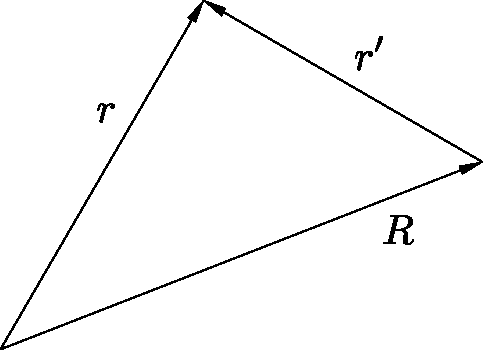
\includegraphics[width=0.3\textwidth]{images/fig_sist_part.pdf}	 
	\end{center}
	\caption{Sistema de partículas}
\end{figure} 

% =================================================================================================
\section{Trabajo en un sistema de partículas}
% =================================================================================================

Empezamos desde
\[
W = W^{ext} + W^{int}
\]
donde el trabajo externo puede escribirse
\notamargen{Quiero un $\ell$ en bold, no me gusta el ${\bf s}$.}
\be
W^{ext} = \sum_i^N \int_1^2 \vb{F}_i^e \cdot d\vb{s}
\label{mc_work_ext}
\ee

La no dependencia del camino para la integral que da \eqref{mc_work_ext} requiere que 
\[
\vb{F}_i^e = \vb{F}_i^e( \vb{r}_i ) \qquad \nabla_{r_i} \times \vb{F}_i^e = 0
\]
y entonces puedo inducir la existencia de una función potencial para las fuerzas externas,
\notamargen{barra resizeable ya.}
\[
W^{ext} = - \sum_i^N  \left. \Delta V_i \right]_1^2 
\]

Por otro lado,
\[
W^{int}_c = \int_1^2 \sum_{\substack{j\\j\neq i}}^N  \vb{F}_{ij}^e \cdot d\vb{s}_i  
\]
\[
\sum_i^N W_i^{int} =  W^{int} = \sum_{\substack{j \\ i\neq j}}^N  \int_1^2 \sum_{\substack{j \\ j\neq i}}^N  \vb{F}_{ij}^e \cdot 
d\vb{s}_i  
\]

% =================================================================================================
\section{Lagrangiano cíclico en el tiempo}
% =================================================================================================

Empecemos desde la derivada total con respecto al tiempo del lagrangiano,
\[
\frac{d}{dt}\left( \Lag( q, \dot{q}, t)\right) = \dpar{\Lag}{q} \dot{q} + \dpar{\Lag}{\dot{q}} \ddot{q} + \dpar{\Lag}{t}
\]
y usando la derivada total del término 
\[
\frac{d}{dt}\left( \dpar{\Lag}{\dot{q}}\dot{q}\right) =
\frac{d}{dt}\left( \dpar{\Lag}{\dot{q}} \right) \dot{q} + \dpar{\Lag}{\dot{q}} \ddot{q} .
\]

Reemplazando una en otra resulta que 
\[
\frac{d}{dt}\left( \Lag( q, \dot{q}, t)\right) = \dpar{\Lag}{q} \dot{q} + \frac{d}{dt}\left( \dpar{\Lag}{\dot{q}}\dot{q}\right) -
\frac{d}{dt}\left( \dpar{\Lag}{\dot{q}} \right) \dot{q} + \dpar{\Lag}{t}
\]
y acomodando un poco
\[
\frac{d}{dt}\left( \Lag( q, \dot{q}, t)\right) = 
\left[ \dpar{\Lag}{q}  - \frac{d}{dt}\left( \dpar{\Lag}{\dot{q}} \right) \right] \dot{q} + 
\frac{d}{dt}\left( \dpar{\Lag}{\dot{q}}\dot{q}\right)  + \dpar{\Lag}{t}
\]
\[
\frac{d}{dt}\left( \Lag( q, \dot{q}, t)\right) = \frac{d}{dt}\left( p \dot{q} \right) + \dpar{\Lag}{t}
\]
y entonces previo pase mágico de términos,
\[
\frac{d}{dt}\left( p\dot{q} - \Lag \right) = -\dpar{\Lag}{t}
\]
y si definimos
\[
\Ham \equiv p\dot{q} - \Lag 
\]
resulta que 
\[
\dtot{\Ham}{t} = - \dpar{\Lag}{t}.
\]

Entonces si el lagrangiano no depende explícitamente del tiempo se tiene que $\Ham = cte.$. Además,
si se cumplen 
\[
T=T_2 \qquad V \neq V(\dot{q})
\]
y además los vínculos no dependen del tiempo se tiene que $\Ham=E$, es decir, el Hamiltoniano es la
energía. La condicion de que los vínculos no dependan del tiempo genera en realidad que $T=T_2$.

Por otro lado $E = cte.$ si $W^{nc} = 0$.

% =================================================================================================
\section{Energía cinética y el hamiltoniano}
% =================================================================================================

Dado que la energía cinética tiene la forma general
\[
T = \underbrace{\frac{1}{2} \sum_i^N m_i \left( \dpar{\vb{r}_i}{t} \right)^2}_{T_0}  +
\underbrace{\sum_j^{3n-k} b_j(q_1,...,q_{3N-k},t)\dot{q}_j  }_{T_1} +
\underbrace{\frac{1}{2} \sum_j^{3n-k}\sum_s^{3n-k}  a_{js}(q_1,...,q_{3N-k},t)\dot{q}_s\dot{q}_j }_{T_2}
\]
entonces se sigue que 
\be
E = T_0 + T_1 + T_2 + V
\label{mc_E}
\ee
y como 
\[
p_i = \dpar{\Lag}{\dot{q}_i} = T_1 + 2T_2 
\]
es 
\[
\Ham = \sum_i^N p_i\dot{q}_i - (T_0 + T_1 + T_2 - V) = 2T_2 + T_1 - T_0 - T_1 - T_2 + V = T_2 - T_0 + V
\]
pero como E es \eqref{mc_E} se tendrá 
\[
E = H \iff 2T_0 + T1 = 0
\]
y un solución de este sistema es, por supuesto, $T_0 = T_1 = 0$

% =================================================================================================
\section{Principio de acción mínima}
% =================================================================================================

También Principio variacional de Hamilton. Partimos de una acción,
\[
S = \int_{t_i}^{t_f} \Lag( q_i, \dot{q}_i, t ) dt \qquad \Lag = T-V
\]

La trayectoria real de un sistema con lagrangiano $\Lag$ es tal que $S$ es mínimo para cualquier 
trayectoria posible entre $q(t=t_i)$ y $q(t=t_f)$. Consideramos una variación con extremos fijos,
es decir 
\[
\delta q(t=t_i) = 0 \qquad \delta q(t=t_f) = 0
\]
y a tiempo fijo $\delta t = 0$. Esto último signfica que todas las trayectorias emplearán el 
mismo tiempo (no se variará).
\notamargen{Cuán sketchi es todo esto!! Mucho para aclarar. Tal vez se justifique un minicurso
de variacional como apéndice.}

\begin{figure}
	\begin{center}
	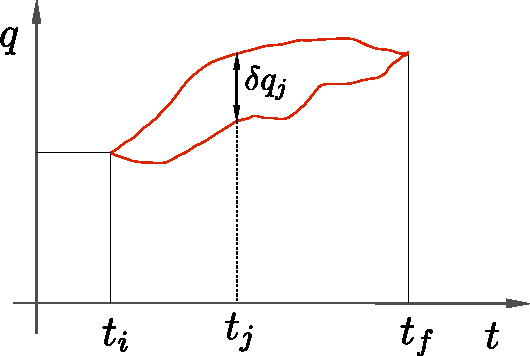
\includegraphics[width=0.4\textwidth]{images/fig_accion.pdf}	 
	\end{center}
	\caption{El principio de acción mínima}
\end{figure}

Consideramos una variación de la integral,
\[
\delta I =  \int_{t_i}^{t_f} \sum_i^N \left( \dpar{\Lag}{\dot{q}_i} \delta \dot{q}_i + \dpar{\Lag}{q_i} \delta q_i  \right) dt,
\]
y notamos que será beneficioso utilizar integración por partes para expresar todo en función de
las variaciones de las coordenadas (las $\delta q_i$), de manera que como
\[
\frac{d}{dt}\left( \dpar{\Lag}{\dot{q}_i} \delta q_i \right) =
\frac{d}{dt}\left( \dpar{\Lag}{\dot{q}_i} \right) \delta q_i + \dpar{\Lag}{\dot{q}_i}\delta \dot{q}_i,
\]
resulta
\[
\delta I =  \int_{t_i}^{t_f} \sum_i^N \left[ \frac{d}{dt}\left( \dpar{\Lag}{\dot{q}_i} \delta q_i \right) -
\frac{d}{dt}\left( \dpar{\Lag}{\dot{q}_i} \right) \delta q_i + \dpar{\Lag}{q_i} \delta q_i  \right] dt,
\]
separamos los dos términos,
\[
\delta I =  \int_{t_i}^{t_f} \sum_i^N \left[ \frac{d}{dt}\left( \dpar{\Lag}{\dot{q}_i} \delta q_i \right) \right] dt -
\int_{t_i}^{t_f} \sum_i^N \left[ \frac{d}{dt}\left( \dpar{\Lag}{\dot{q}_i} \right) - \dpar{\Lag}{q_i} 
\right]  \delta q_i  dt,
\]
y resulta que el primero por el teorema fundamental del cálculo es
\be
\int_{t_i}^{t_f} \sum_i^N \left[ \frac{d}{dt}\left( \dpar{\Lag}{\dot{q}_i} \delta q_i \right) \right] dt =
\left. \dpar{\Lag}{\dot{q}_i} \delta q_i\right|_{t_i}^{t_f}
\label{mc_borde_term}
\ee
y es nulo porque $\delta q_i=0$ en los extremos (recordemos que las variaciones son nulas en los extremos de
integración). Decimos que este es un término de superficie.
Entonces
\[
\delta I =  -\int_{t_i}^{t_f} \sum_i^N \left[ \frac{d}{dt}\left( \dpar{\Lag}{\dot{q}_i} \right) - \dpar{\Lag}{q_i} 
\right]  \delta q_i  dt = 0
\]
se verificará por el cumplimiento de las ecuaciones de Euler-Lagrange
\[
\sum_i^N  \left[ \frac{d}{dt}\left( \dpar{\Lag}{\dot{q}_i} \right) - \dpar{\Lag}{q_i} \right] = 0.
\]

Luego, si se hace $\Lag' = \Lag + df/dt$ (ambos lagrangianos difieren en una derivada total con 
respecto al tiempo) la trayectoria que minimiza $\Lag'$ es la que misma que minimiza
$\Lag$ por la condición dada por \eqref{mc_borde_term}. Entonces 
\[
\delta S = 0 \iff \sum_i^N  \left[ \frac{d}{dt}\left( \dpar{\Lag}{\dot{q}_i} \right) - \dpar{\Lag}{q_i} \right] = 0.
\]

La moraleja es que si los lagrangianos difieren en una derivada total del tiempo obtenemos la misma
física.

% =================================================================================================
\section{Aplicaciones del principio de acción mínima}
% =================================================================================================

\[
S = \int (T-V_0) dt
\]
donde el lagrangiano es con $V=V_0$ constante (un lagrangiano sujeto a potencial constante).
La integral de acción da una medida de la longitud de la órbita (el espacio recorrido).
Para una partícula sujeta a $V=0$
\[
S = \frac{1}{2}\int m v_0^2 dt = \frac{1}{2}mv_0^2(t-t_0)
\]
de manera que $v_0(t-t_0)$ representa la distancia $d$ recorrida, y es 
\[
S = \frac{1}{2}mv_0 d
\]

Comentario sobre el cálculo de las variaciones
\notamargen{Esta idea debe estar en el suplemento matemático que le dedicaremos a variacional}
\[
I = \int f\left(x, \dtot{x}{t}, t\right) dt 
\]
entonces $I$ es extremo si
\[
\frac{d}{dt} \left( \dpar{f}{[dx/dt]}\right) - \dpar{f}{x} = 0
\]
También podemos encontrar esta notación, dependiendo del tipo de problema,
\[
I = \int f\left(y, \dtot{y}{x}, x\right) dx 
\]


% =================================================================================================
\section{Multiplicadores de Lagrange}
% =================================================================================================

Partimos de la acción
\[
S = \int_{t_i}^{t_f} \Lag \left( q_i[t], \dot{q}_i[t], t \right) dt
\]
entonces 
\[
\delta S = 0 \quad \Leftrightarrow \quad \int
\sum_{j=1}^{N} \left[ \frac{d}{dt}\left( \dpar{\Lag}{\dot{q}_j} \right) -\dpar{\Lag}{q_j} \right]\delta q_j dt
\]
donde $\delta q_j$ son desplazamientos independientes. Si no se pued despejar alguna $\delta q_j$ (con 
vínculos no-holónomos, por ejemplo) entonces algún $\delta q_j$ es independiente de modo que para que 
valga $\delta S =0 $ necesitaré 
\[
\sum_{\ell}^N a_\ell^k(q_i,t) \dot{q}_\ell + b^k(q_i,t) = 0
\]
que son los vínculos ($k=1,...,s$); son $s$ ecuaciones de vínculo.
Multiplicamos por $\delta t$ y vemos que no son independientes
\[
\sum_{\ell}^N a_\ell^k(q_i,t) \delta {q}_\ell + b^k(q_i,t) \delta t= 0
\]

Sean $\delta q_\ell$ variación a $t$ fijo, entonces 
\[
\sum_{\ell}^N a_\ell^k(q_i,t) \delta {q}_\ell
\]
\[
\int_{t_i}^{t_f} \lambda^k \sum_{\ell}^N a_\ell^k(q_i,t) \delta {q}_\ell dt = 0
\]
recordando que $\ell$ suma en los grados de libertad. Podemos sacar la suma fuera,
\[
\sum_{k}^s \int_{t_i}^{t_f} \lambda^k \sum_{\ell}^N a_\ell^k(q_i,t) \delta {q}_\ell dt = 0
\]
Absorbo la otra sumatoria en el segundo término y paso de $\ell \to j$.
\[
\int  \sum_{j=1}^N \left\{ \frac{d}{dt}\left( \dpar{\Lag}{\dot{q}_j} \right) -\dpar{\Lag}{q_j}
- \sum_{k}^s \lambda^k a_\ell^k(q_i,t) \right\} \delta {q}_\ell dt = 0
\]
entonces 
\[
\sum_{j=1}^N \frac{d}{dt}\left( \dpar{\Lag}{\dot{q}_j} \right) -\dpar{\Lag}{q_j} =
\sum_{j=1}^N \sum_{k}^s \lambda^k a_\ell^k(q_i,t) =  
\sum_{j=1}^N \sum_{k}^s \lambda^k \nabla_j f^k \cdot \frac{\delta \vb{r}_j}{\delta q_j} 
\]
siendo $\nabla_j f^k $ el gradiente de la ecuación de víngulo respeco de $j$ y donde $\lambda^k$
es la fuerza de vínculo asociada al vínculo no despejado pues como la fuerza generalizada
(que no proviene de potencial)
\[
Q_j = \sum_i^N \vb{F}_i^a \cdot \dpar{\vb{r}_i}{q_j}
\]
y comparando vemos que 
\[
Q_j = \sum \lambda^k a^k_j(q_j,t) \quad \textrm{vínculos no holónomos}
\]
\[
Q_j=  \sum \lambda^k \nabla_j f^k \cdot \delta \vb{r}_j  \quad \textrm{vínculos holónomos}
\]

En el caso de vínculos holónomos 
\[
g(\vb{r}_1,...,\vb{r}_n,t) = 0 
\]
donde no quise despejar en función de $q_q,...,q_n$ resulta que 
\notamargen{El supraíndice con $\delta q_j$ va sobre el igual en realidad.}
\[
Q_j^{\delta q_j} =  \sum_i^N \lambda (\nabla_i f^k\cdot\delta\vb{r}_i)
\]
donde $\delta\vb{r}_i$ es un desplazamiento virtual de la partícula.
Vamos a reescribir este término,
\[
\sum_i^N \dpar{g^k}{\vb{r}_i} \delta \vb{r}_i = 0
\]
\[
\nabla_i f^k\cdot\delta\vb{r}_i = \sum_i \dpar{g^k}{\vb{r}_i} \dpar{\vb{r}_i}{q_j} \delta q_j
\]
\[
Q_j^{\delta q_j} =  \lambda \sum_k \dpar{g^k}{\vb{r}_i} \sum_j \dpar{\vb{r}_i}{q_j} \delta q_j
\]
luego como 
\[
a^k_j \equiv \dpar{g^k}{\vb{r}_i}
\]
se sigue que los $\lambda^k$ son las fuerzas de vínculo.

En el caso de vínculos no holónomos $\lambda^k$ son las fuerzas de vínculo asociadas a los 
vínculos no retirados.

\[
Q_j {\delta q_j} =  \sum \lambda^k (\nabla_i g^k\cdot\delta\vb{r}_i)
\]
\[
Q_j =  \sum_k \lambda^k \dpar{g^k}{\vb{r}_i} \dpar{\vb{r}_i}{q_j}
\]
\[
Q_j =  \sum_k \lambda^k \dpar{g^k}{q_j}
\]
entonces $\lambda^k=F^v$.

Como extra escribamos que para cada grado de libertad $j$ 
\[
\dpar{\Lag}{q_j} - \frac{d}{dt}\left( \dpar{\Lag}{\dot{q}_j} \right) - \sum_k^s \lambda^k a_j^k \equiv 0
\]
donde $\delta q_j$ son ahora independientes.
\[
Q_j = \sum_i^N F_i^a \dpar{\vb{r}_i}{q_j}. 
\]

\begin{ejemplillo}{\bf Moneda rodando por un plano}
Consideramos una moneda que rueda libremente por un plano (no sujeta a potencial).
\[
	\vb{V}_{cm} = -\vb{\Omega} \times \vb{r} =
	-(\dot{\phi}\hat{2} + \dot{\psi}\hat{3}) \times (-a\hat{2})
\]
\[
	\dot{x}\hat{x} + \dot{y}\hat{y} = -a \dot{\psi}\hat{1}
\]
siendo los vínculos
\[
	z_{cm} - a = 0 \qquad \theta=\pi/2 \qquad |\vb{V}_{cm}| = a\dot{\psi}
\]
de tal modo que son dos grados de libertad. El lagrangiano puede escribirse como 
\[
	\Lag = T = \frac{1}{2}m a^2 \dot{\psi}^2  + \frac{1}{2} I_2^2 \dot{\phi}^2 + \frac{1}{2} I_3^2\dot{\psi}^2
\]
\notamargen{No entiendo/recuerdo lo que quise decir con la expresión {\it bajar los ejes}.
Calculo que se relaciona con la proyección de los ejes 123 en xyz. Confirmarlo.}

Como los vínculos dependen de la velocidad, resulta 
\[
\dot{y} = a\dot{\psi} \cos(\psi) \sin(\phi) = a \sin(\phi) \dot{\psi}
\]
\[
\dot{x} = a\dot{\psi} \cos(\psi) \cos(\phi) = a \cos(\phi) \dot{\psi}
\]
de tal manera que 
\[
	\dot{y} - a \sin(\phi) \dot{\psi} = 0 \qquad \dot{x} - a \cos(\phi) \dot{\psi} = 0
\]
y luego esto equivale a 
\[
	\lambda_1(dy - a \sin(\phi) d\psi) = 0 \qquad \lambda_2(dx - a \cos(\phi) d\psi)= 0
\]
y finalmente 
\[
	\frac{d}{dt}\left(\dpar{\Lag}{\dot{q}_i}\right) - \dpar{\Lag}{q_i} =
	\lambda_i \nabla_i f \cdot \delta \vb{r}_i
\]
Podemos escribir
\[
	m \ddot{x} = \lambda_1 \qquad m \ddot{x} = m a \frac{d}{dt}( \cos(\phi)\dot{\psi} )
\]
\[
	m \ddot{x} = m a ( -\sin(\phi)\dot{\phi}\dot{\psi} + \cos(\phi)\ddot{\psi} )
\]
\[
	m \ddot{y} = \lambda_2
\]
\[
	I_2\ddot{\phi} = 0 \qquad I_3\ddot{\psi} = - \lambda_2 a \sin(\phi) -\lambda_1 a \cos(\phi)
\]
\[
	\hat{1} = \cos(\psi)[\sin(\phi)\hat{y} + \cos(\phi)\hat{x}]
\]

\label{moneda}
\end{ejemplillo}

% ============================================================================


\bibliographystyle{CBFT-apa-good}	% (uses file "apa-good.bst")
\bibliography{CBFT.Referencias} % La base de datos bibliográfica

\end{document}
